\documentclass[]{article}
\usepackage[T1]{fontenc}
\usepackage{lmodern}
\usepackage{amssymb,amsmath}
\usepackage{ifxetex,ifluatex}
\usepackage{fixltx2e} % provides \textsubscript
% Set line spacing
% use upquote if available, for straight quotes in verbatim environments
\IfFileExists{upquote.sty}{\usepackage{upquote}}{}
\ifnum 0\ifxetex 1\fi\ifluatex 1\fi=0 % if pdftex
  \usepackage[utf8]{inputenc}
\else % if luatex or xelatex
  \ifxetex
    \usepackage{mathspec}
    \usepackage{xltxtra,xunicode}
  \else
    \usepackage{fontspec}
  \fi
  \defaultfontfeatures{Mapping=tex-text,Scale=MatchLowercase}
  \newcommand{\euro}{€}
\fi
% use microtype if available
\IfFileExists{microtype.sty}{\usepackage{microtype}}{}
\usepackage[margin=1in]{geometry}
\usepackage{color}
\usepackage{fancyvrb}
\newcommand{\VerbBar}{|}
\newcommand{\VERB}{\Verb[commandchars=\\\{\}]}
\DefineVerbatimEnvironment{Highlighting}{Verbatim}{commandchars=\\\{\}}
% Add ',fontsize=\small' for more characters per line
\usepackage{framed}
\definecolor{shadecolor}{RGB}{248,248,248}
\newenvironment{Shaded}{\begin{snugshade}}{\end{snugshade}}
\newcommand{\KeywordTok}[1]{\textcolor[rgb]{0.13,0.29,0.53}{\textbf{{#1}}}}
\newcommand{\DataTypeTok}[1]{\textcolor[rgb]{0.13,0.29,0.53}{{#1}}}
\newcommand{\DecValTok}[1]{\textcolor[rgb]{0.00,0.00,0.81}{{#1}}}
\newcommand{\BaseNTok}[1]{\textcolor[rgb]{0.00,0.00,0.81}{{#1}}}
\newcommand{\FloatTok}[1]{\textcolor[rgb]{0.00,0.00,0.81}{{#1}}}
\newcommand{\CharTok}[1]{\textcolor[rgb]{0.31,0.60,0.02}{{#1}}}
\newcommand{\StringTok}[1]{\textcolor[rgb]{0.31,0.60,0.02}{{#1}}}
\newcommand{\CommentTok}[1]{\textcolor[rgb]{0.56,0.35,0.01}{\textit{{#1}}}}
\newcommand{\OtherTok}[1]{\textcolor[rgb]{0.56,0.35,0.01}{{#1}}}
\newcommand{\AlertTok}[1]{\textcolor[rgb]{0.94,0.16,0.16}{{#1}}}
\newcommand{\FunctionTok}[1]{\textcolor[rgb]{0.00,0.00,0.00}{{#1}}}
\newcommand{\RegionMarkerTok}[1]{{#1}}
\newcommand{\ErrorTok}[1]{\textbf{{#1}}}
\newcommand{\NormalTok}[1]{{#1}}
\usepackage{graphicx}
% Redefine \includegraphics so that, unless explicit options are
% given, the image width will not exceed the width of the page.
% Images get their normal width if they fit onto the page, but
% are scaled down if they would overflow the margins.
\makeatletter
\def\ScaleIfNeeded{%
  \ifdim\Gin@nat@width>\linewidth
    \linewidth
  \else
    \Gin@nat@width
  \fi
}
\makeatother
\let\Oldincludegraphics\includegraphics
{%
 \catcode`\@=11\relax%
 \gdef\includegraphics{\@ifnextchar[{\Oldincludegraphics}{\Oldincludegraphics[width=\ScaleIfNeeded]}}%
}%
\ifxetex
  \usepackage[setpagesize=false, % page size defined by xetex
              unicode=false, % unicode breaks when used with xetex
              xetex]{hyperref}
\else
  \usepackage[unicode=true]{hyperref}
\fi
\hypersetup{breaklinks=true,
            bookmarks=true,
            pdfauthor={Thomas Rost},
            pdftitle={BN - Assignment 2},
            colorlinks=true,
            citecolor=blue,
            urlcolor=blue,
            linkcolor=magenta,
            pdfborder={0 0 0}}
\urlstyle{same}  % don't use monospace font for urls
\setlength{\parindent}{0pt}
\setlength{\parskip}{6pt plus 2pt minus 1pt}
\setlength{\emergencystretch}{3em}  % prevent overfull lines
\setcounter{secnumdepth}{5}

%%% Change title format to be more compact
\usepackage{titling}
\setlength{\droptitle}{-2em}
  \title{BN - Assignment 2}
  \pretitle{\vspace{\droptitle}\centering\huge}
  \posttitle{\par}
  \author{Thomas Rost}
  \preauthor{\centering\large\emph}
  \postauthor{\par}
  \predate{\centering\large\emph}
  \postdate{\par}
  \date{Saturday, December 13, 2014}




\begin{document}

\maketitle


{
\hypersetup{linkcolor=black}
\setcounter{tocdepth}{2}
\tableofcontents
}
\newpage

\section{comparison of two learning
algos}\label{comparison-of-two-learning-algos}

\subsection{1: data discretization}\label{data-discretization}

Investigate what is the effect of data discretisation on the structure
of the learnt Bayesian network, e.g., in terms of number of arcs,
changes in arc direction, etc., by considering three discretisations of
the continuous features in the iris dataset with different number of
bins (see Section B.3). Do this for both classes of learning algorithms
and compare the results.

Discretizing the iris data set with the hartemink algorithm leads to the
networks shown in the figures below. The first three depict a
score-based algorithm, while the second triple shows the effect of
discretization on constraint-based algorithms. \#\#\#General
considerations: The best way to deal with data is case dependent. In the
case of discretization, some Datasets might benefit from more bins while
others benefit from less, depending on the distribution of the variables
within the set. In the case of the iris data set, a bin number of three
seems to be a sensible choice, given the three speicies. When looking at
the plots, we can see that both petal width and petal length can be
binned in three bins with only minor overlap between the species.
However, sepal length and width have a big overlap and might benefit
from higher bin numbers. We considered three, five and seven bins for
both score and constraint based algorithms.

\subsubsection{Score Based:}\label{score-based}

Three bins leads to four arcs with relatively sensible directions:
species influences petal length which influences sepal length, seepal
width influences petal width which in turn influences speices. The graph
is well-connected, each variable will play a role in classifying the
species, even if two of them are indirect. The causality seems a bit
odd, but not completely against intuition. All arcs are directed.

five bins leads to four arcs with different causality compared to three
bins: sepal length now influences petal length which influences petal
width which influences species which in turn influences sepal width. On
a first glance, the causality in the three bins case seems to make more
sense, but again the logic does not ddefy intuition on a disturbing
level. All arcs are directed.

seven bins also leads to four arcs. The causality in this case seems
different to the others at least in two major ways: Species is a leaf
and one node (petal width) has two children, compared to the one on one
mapping of parents to children in the previous sections. The logic in
this cacse seems weaker compared to the other two bin number cases,
since species should have a more direct influence to sepal width.

\begin{Shaded}
\begin{Highlighting}[]
\KeywordTok{plot}\NormalTok{(iris)}
\end{Highlighting}
\end{Shaded}

\begin{figure}[htbp]
\centering
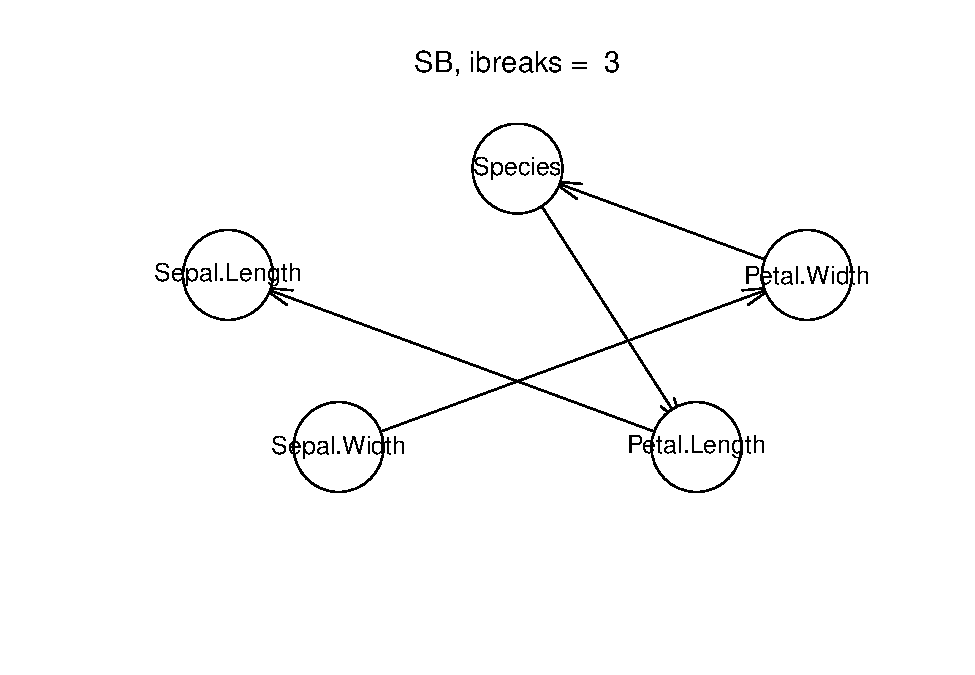
\includegraphics{BN_Ass2_files/figure-latex/unnamed-chunk-2-1.pdf}
\caption{SB , ibreaks = 3}
\end{figure}

\begin{Shaded}
\begin{Highlighting}[]
\NormalTok{for( bins in }\KeywordTok{c}\NormalTok{(}\DecValTok{3}\NormalTok{,}\DecValTok{5}\NormalTok{,}\DecValTok{7}\NormalTok{))\{}
\NormalTok{tmp=}\KeywordTok{discretize}\NormalTok{(iris[-}\DecValTok{5}\NormalTok{], }\DataTypeTok{method =} \StringTok{'hartemink'}\NormalTok{,}\DataTypeTok{ibreaks=}\NormalTok{bins) }
\NormalTok{NewIris =}\StringTok{ }\KeywordTok{cbind}\NormalTok{(tmp,iris[}\DecValTok{5}\NormalTok{]) }

\NormalTok{IrisNetsb <-}\StringTok{ }\KeywordTok{tabu}\NormalTok{(NewIris)}

\NormalTok{numNodes =}\StringTok{ }\KeywordTok{length}\NormalTok{(IrisNetsb$nodes)}
\NormalTok{numArcs =}\StringTok{ }\KeywordTok{length}\NormalTok{(IrisNetsb$arcs[,}\DecValTok{1}\NormalTok{])}

\KeywordTok{plot}\NormalTok{(IrisNetsb, }\DataTypeTok{font.main =} \DecValTok{1}\NormalTok{, }\DataTypeTok{main =} \KeywordTok{paste}\NormalTok{(}\StringTok{"SB, ibreaks = "}\NormalTok{, bins, }\StringTok{"number of nodes:"} \NormalTok{, numNodes, }\StringTok{"bumber of arcs:"} \NormalTok{, numArcs))}




\NormalTok{\}}
\end{Highlighting}
\end{Shaded}

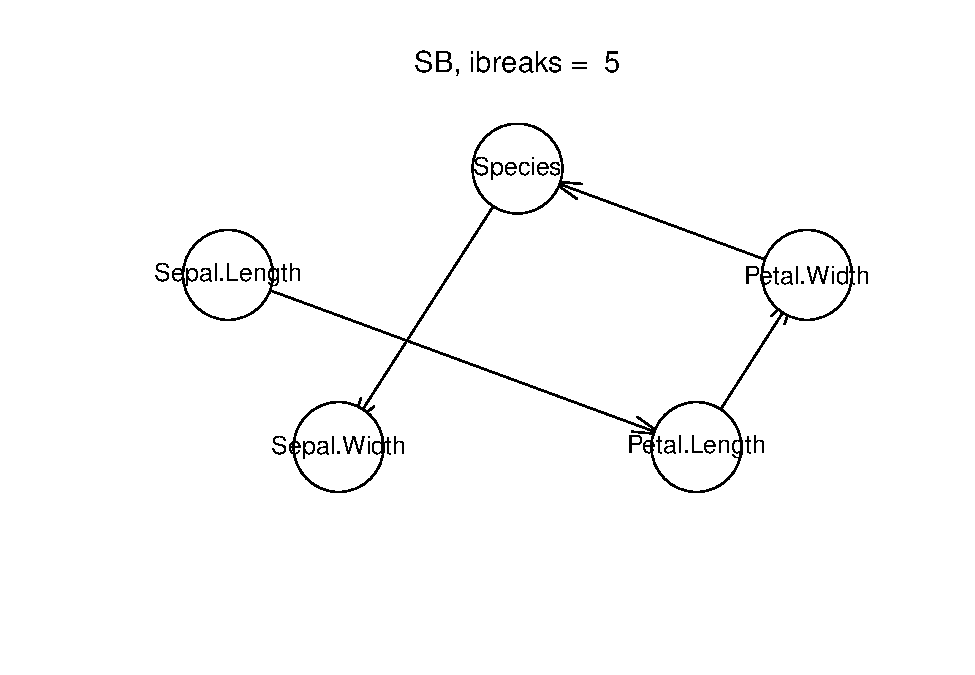
\includegraphics{BN_Ass2_files/figure-latex/unnamed-chunk-2-2.pdf}
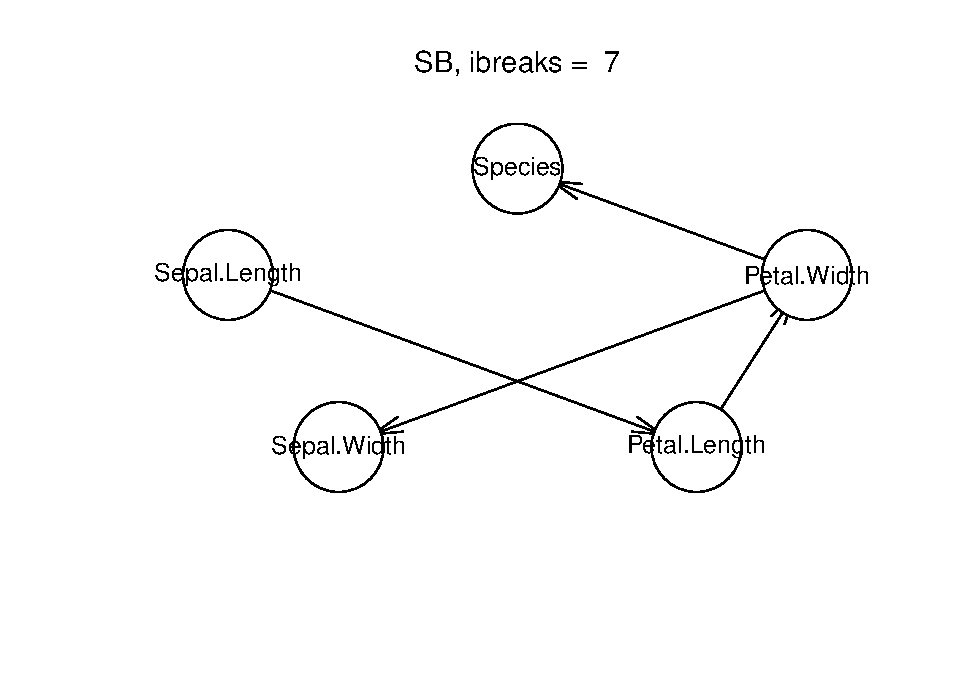
\includegraphics{BN_Ass2_files/figure-latex/unnamed-chunk-2-3.pdf}
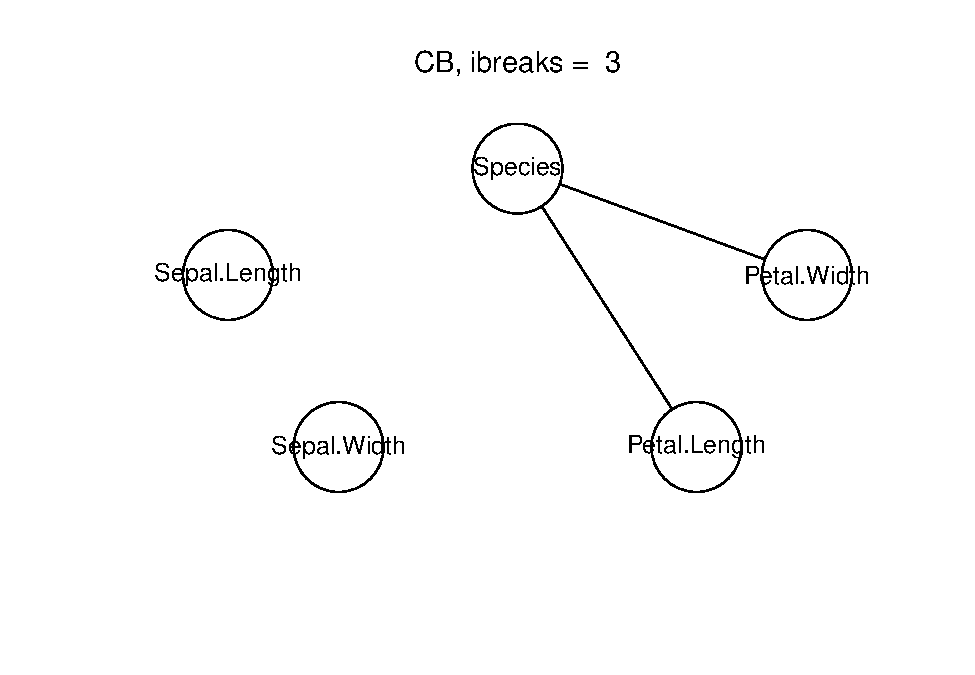
\includegraphics{BN_Ass2_files/figure-latex/unnamed-chunk-2-4.pdf}
\#\#\#Constraint based:

general statement. Constraint based algorithms (all of them were tried
out, although only one is reported here) tend to lead to way less
expressive networks. often arcs are undirected and the number of graphs
is often significantly lower than with score based algorithms. However,
this does not necessarily mean that constraint based algorithms are
``worse''. The constraint nature leads to more robust predictions. the
strengths of the two algorithm classes should be considered for each
task individually. (see Bayesian Probabilities for Constraint-based
Causal Discovery Tom Claassen and Tom Heskes Radboud University Nijmegen
Netherlands). in order to compare score based and constraint based
algorithms, in some cases the cextend() function has been used.

three bins: only two arcs, between petal width and petal length. No
directions. sepal length and width are separate networks that aren't
connected to species.

five bins: four arcs corresponding to the five bins score based
algoriuthm's outcome.

seven bins: three arcs, only connection between species and another node
is petal width. The rest is a separate network.

\begin{Shaded}
\begin{Highlighting}[]
\NormalTok{for( bins in }\KeywordTok{c}\NormalTok{(}\DecValTok{3}\NormalTok{,}\DecValTok{5}\NormalTok{,}\DecValTok{7}\NormalTok{))\{}
\NormalTok{tmp=}\KeywordTok{discretize}\NormalTok{(iris[-}\DecValTok{5}\NormalTok{], }\DataTypeTok{method =} \StringTok{'hartemink'}\NormalTok{,}\DataTypeTok{ibreaks=}\NormalTok{bins) }
\NormalTok{NewIris =}\StringTok{ }\KeywordTok{cbind}\NormalTok{(tmp,iris[}\DecValTok{5}\NormalTok{]) }

\NormalTok{IrisNetcb <-}\StringTok{ }\KeywordTok{iamb}\NormalTok{(NewIris)}
\NormalTok{IrisNetcb2 <-}\StringTok{ }\KeywordTok{cextend}\NormalTok{(IrisNetcb)}

\NormalTok{numNodes =}\StringTok{ }\KeywordTok{length}\NormalTok{(IrisNetcb$nodes)}
\NormalTok{numArcs =}\StringTok{ }\KeywordTok{length}\NormalTok{(IrisNetcb$arcs[,}\DecValTok{1}\NormalTok{])}

\KeywordTok{plot}\NormalTok{(IrisNetcb2, }\DataTypeTok{font.main =} \DecValTok{1}\NormalTok{, }\DataTypeTok{main =} \KeywordTok{paste}\NormalTok{(}\StringTok{"CB, ibreaks = "}\NormalTok{, bins,  }\StringTok{"number of nodes:"} \NormalTok{, numNodes, }\StringTok{"bumber of arcs:"} \NormalTok{, numArcs))}






\NormalTok{\}}
\end{Highlighting}
\end{Shaded}

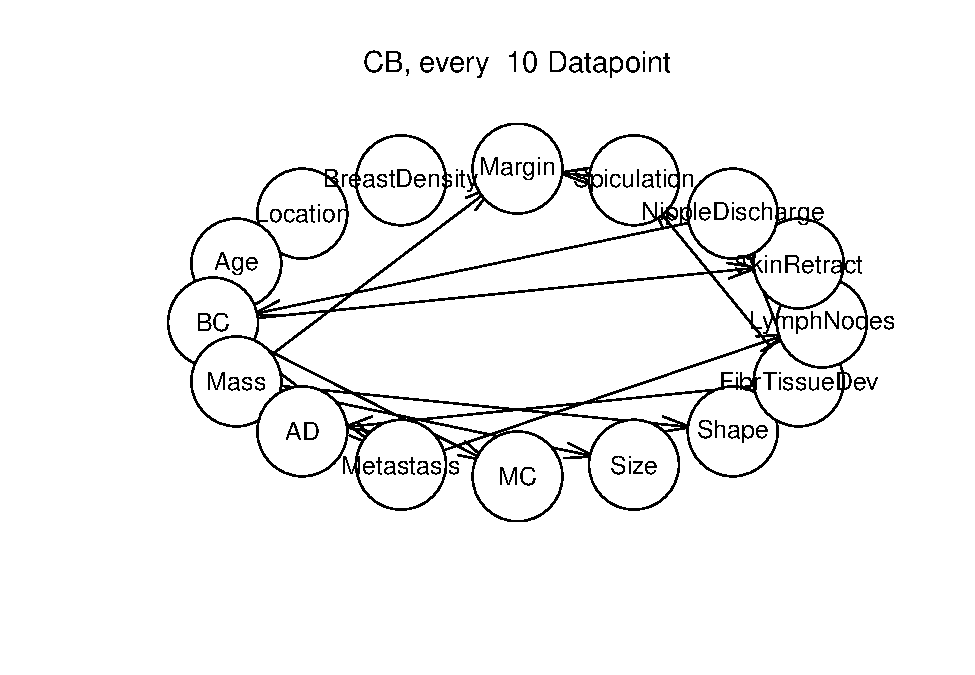
\includegraphics{BN_Ass2_files/figure-latex/unnamed-chunk-3-1.pdf}
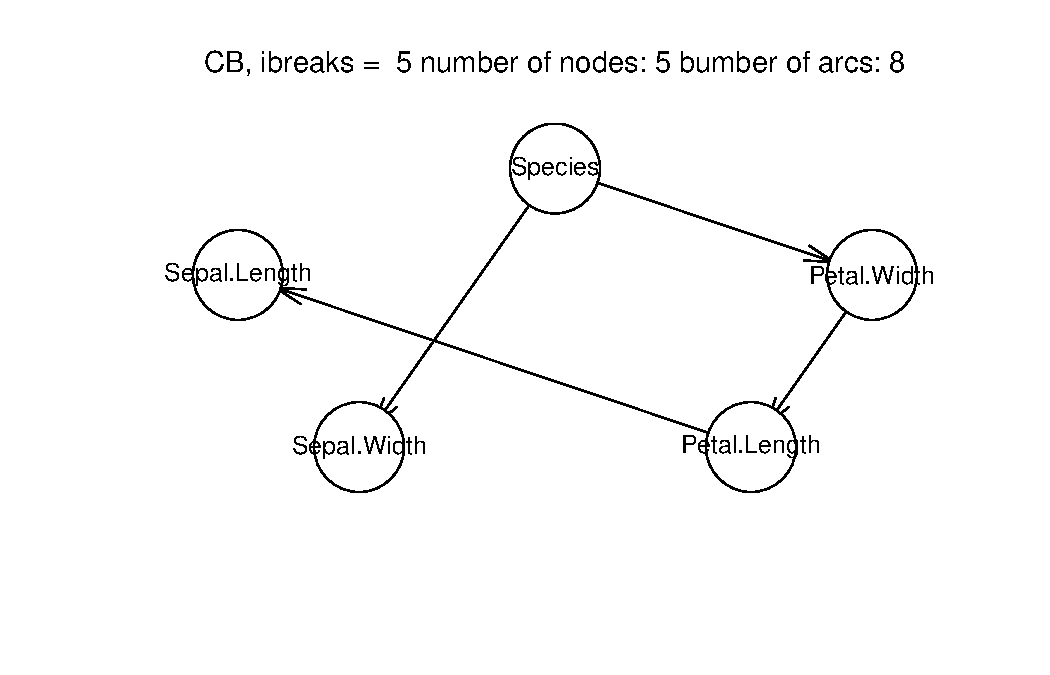
\includegraphics{BN_Ass2_files/figure-latex/unnamed-chunk-3-2.pdf}
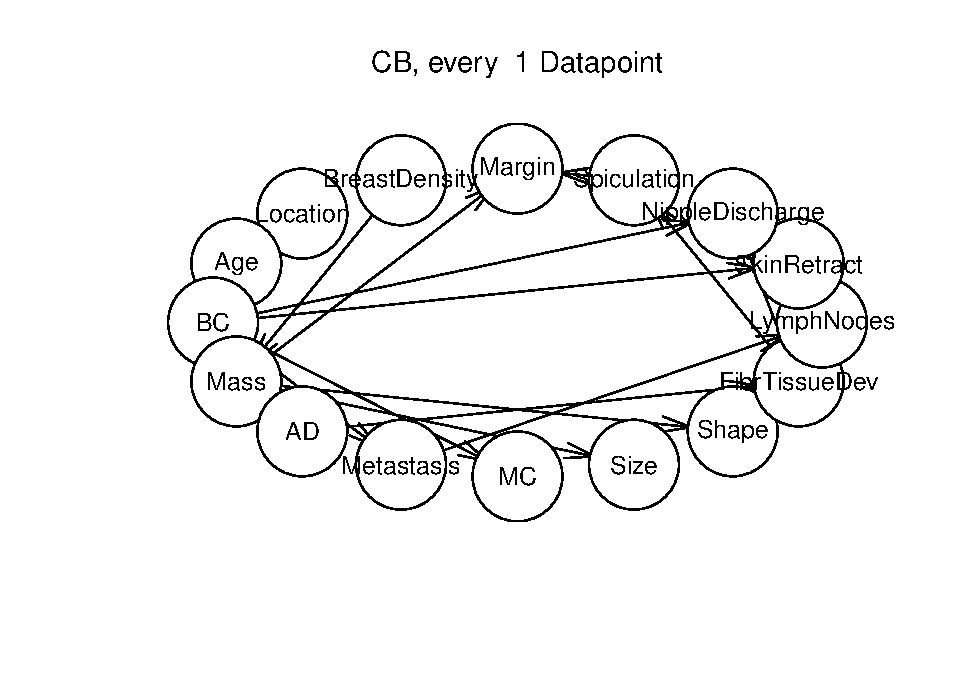
\includegraphics{BN_Ass2_files/figure-latex/unnamed-chunk-3-3.pdf}

\clearpage

\subsection{2: size of dataset}\label{size-of-dataset}

Investigate what is the effect of the size of the dataset on the
structure of the learnt Bayesian network by considering three subsets of
the breast cancer dataset with different number of samples. Do this for
both classes of learning algorithms and compare the results.

\subsubsection{general disclaimer:}\label{general-disclaimer}

again, the constraint based algorithms do not always lead to directed
nodes. the same function has been used as before. The effect of number
of training examples on performance of the training algorithms has been
examined. every tenth data point, half of the data and the full data set
have been examined.

\subsubsection{SB}\label{sb}

for score based algorithms, there is no difference between models
whether the full or the half data set is used. The number of arcs and
arc direction are the same. However, when only a tenth of the data set
has been used, two arcs were not inferred. This seems to be in line with
the idea that more training data generates more sophisticated models.

\subsubsection{CB}\label{cb}

for constraint based algorithms, evaluation of node direction is
complicated. Therefore the discussion will be only for arc number.
Again, no difference in arc number for full or half data set, however, a
node is missing in the tenth-dataset-model. Again, this seems to match
intuition.

\begin{Shaded}
\begin{Highlighting}[]
\NormalTok{a <-}\StringTok{ }\KeywordTok{read.csv}\NormalTok{(}\StringTok{'bc.csv'}\NormalTok{)}

\CommentTok{#plot(a)}

\NormalTok{for(part in }\KeywordTok{c}\NormalTok{(}\DecValTok{10}\NormalTok{,}\DecValTok{2}\NormalTok{,}\DecValTok{1}\NormalTok{))\{}
    \NormalTok{ind =}\StringTok{ }\KeywordTok{sample}\NormalTok{(}\DecValTok{1}\NormalTok{:(}\KeywordTok{nrow}\NormalTok{(a)/part))}
    \NormalTok{BC <-}\StringTok{ }\NormalTok{a[ind,]}
    
    \NormalTok{BC_sbl <-}\StringTok{ }\KeywordTok{tabu}\NormalTok{(BC)}
    
    
\NormalTok{numNodes =}\StringTok{ }\KeywordTok{length}\NormalTok{(BC_sbl$nodes)}
\NormalTok{numArcs =}\StringTok{ }\KeywordTok{length}\NormalTok{(BC_sbl$arcs[,}\DecValTok{1}\NormalTok{])}
    
    
    \KeywordTok{plot}\NormalTok{(BC_sbl , }\DataTypeTok{font.main =} \DecValTok{1}\NormalTok{, }\DataTypeTok{main =} \KeywordTok{paste}\NormalTok{(}\StringTok{"SB, every "}\NormalTok{, part, }\StringTok{"Datapoint"}\NormalTok{, bins,  }\StringTok{"number of nodes:"} \NormalTok{, numNodes, }\StringTok{"bumber of arcs:"} \NormalTok{, numArcs))}

    
\NormalTok{\}}
\end{Highlighting}
\end{Shaded}

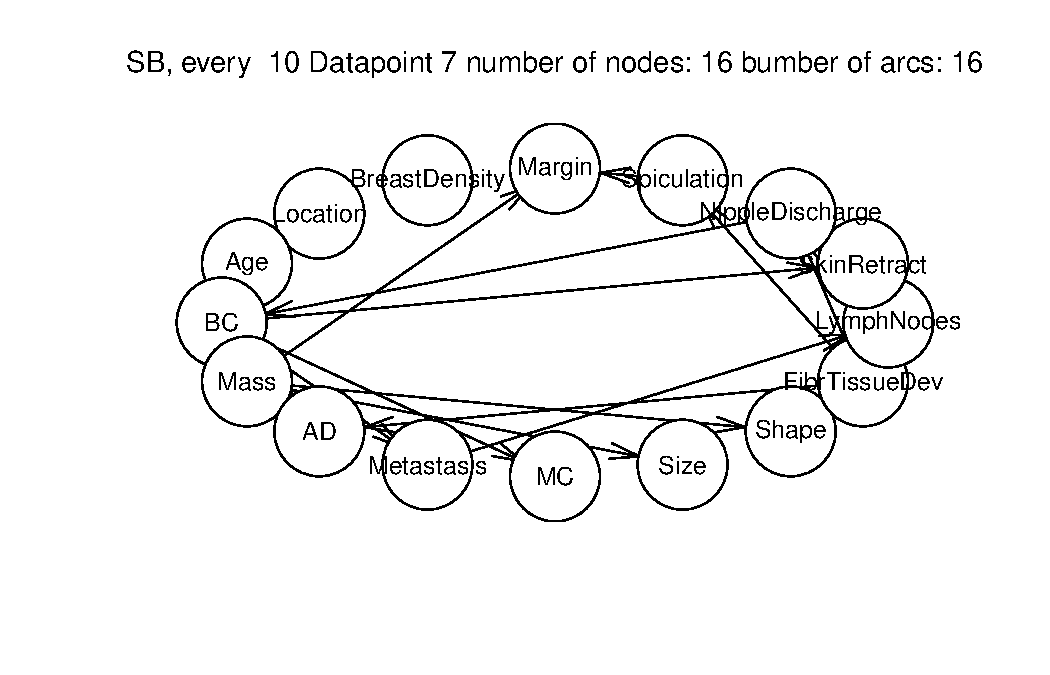
\includegraphics{BN_Ass2_files/figure-latex/unnamed-chunk-4-1.pdf}
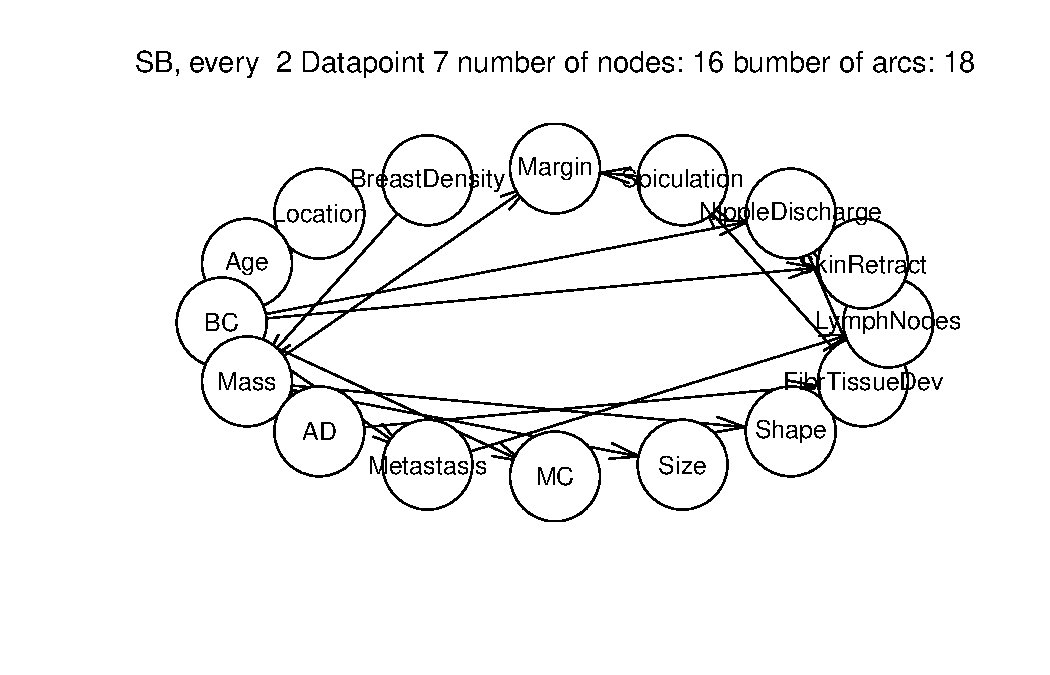
\includegraphics{BN_Ass2_files/figure-latex/unnamed-chunk-4-2.pdf}
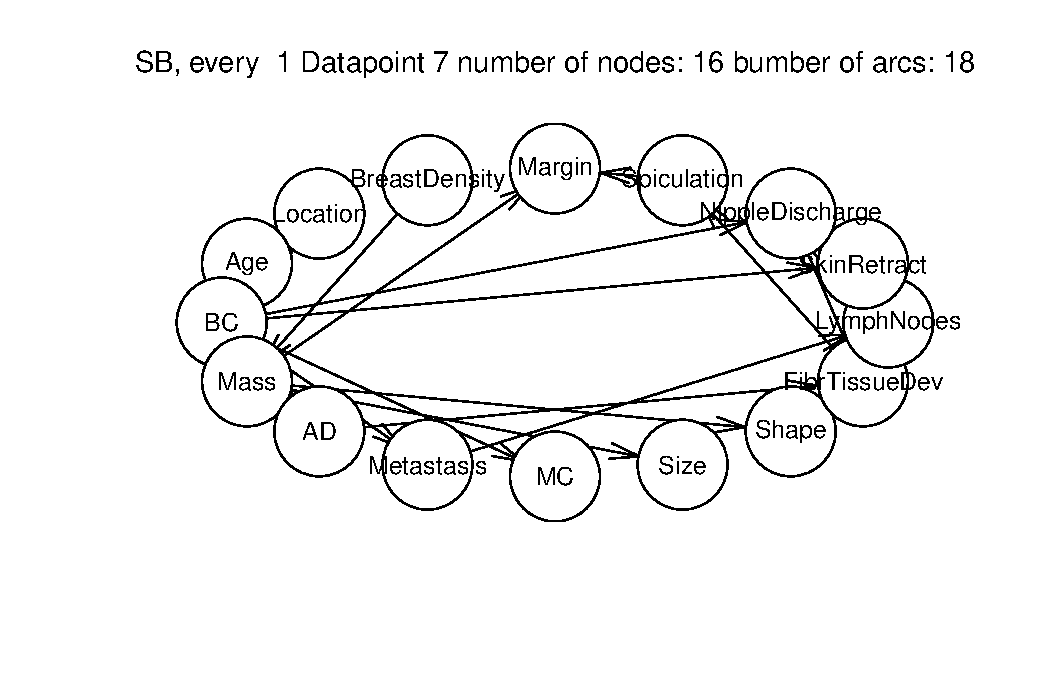
\includegraphics{BN_Ass2_files/figure-latex/unnamed-chunk-4-3.pdf}

\begin{Shaded}
\begin{Highlighting}[]
\NormalTok{for(part in }\KeywordTok{c}\NormalTok{(}\DecValTok{1}\NormalTok{,}\DecValTok{2}\NormalTok{,}\DecValTok{10}\NormalTok{))\{}
    \NormalTok{ind =}\StringTok{ }\KeywordTok{sample}\NormalTok{(}\DecValTok{1}\NormalTok{:(}\KeywordTok{nrow}\NormalTok{(a)/part))}
    \NormalTok{BC <-}\StringTok{ }\NormalTok{a[ind,]}
    
    \NormalTok{BC_cbl <-}\StringTok{ }\KeywordTok{iamb}\NormalTok{(BC)}
    \NormalTok{BC_cbl2 <-}\StringTok{ }\KeywordTok{cextend}\NormalTok{(BC_sbl)}
    \NormalTok{numNodes =}\StringTok{ }\KeywordTok{length}\NormalTok{(BC_cbl$nodes)}
    \NormalTok{numArcs =}\StringTok{ }\KeywordTok{length}\NormalTok{(BC_cbl$arcs[,}\DecValTok{1}\NormalTok{])}

    \KeywordTok{plot}\NormalTok{(BC_cbl2,  }\DataTypeTok{font.main =} \DecValTok{1}\NormalTok{, }\DataTypeTok{main =} \KeywordTok{paste}\NormalTok{(}\StringTok{"CB, every "}\NormalTok{, part, }\StringTok{"Datapoint"}\NormalTok{, bins,  }\StringTok{"number of nodes:"} \NormalTok{, numNodes, }\StringTok{"bumber of arcs:"} \NormalTok{, numArcs))}

    

\NormalTok{\}}
\end{Highlighting}
\end{Shaded}

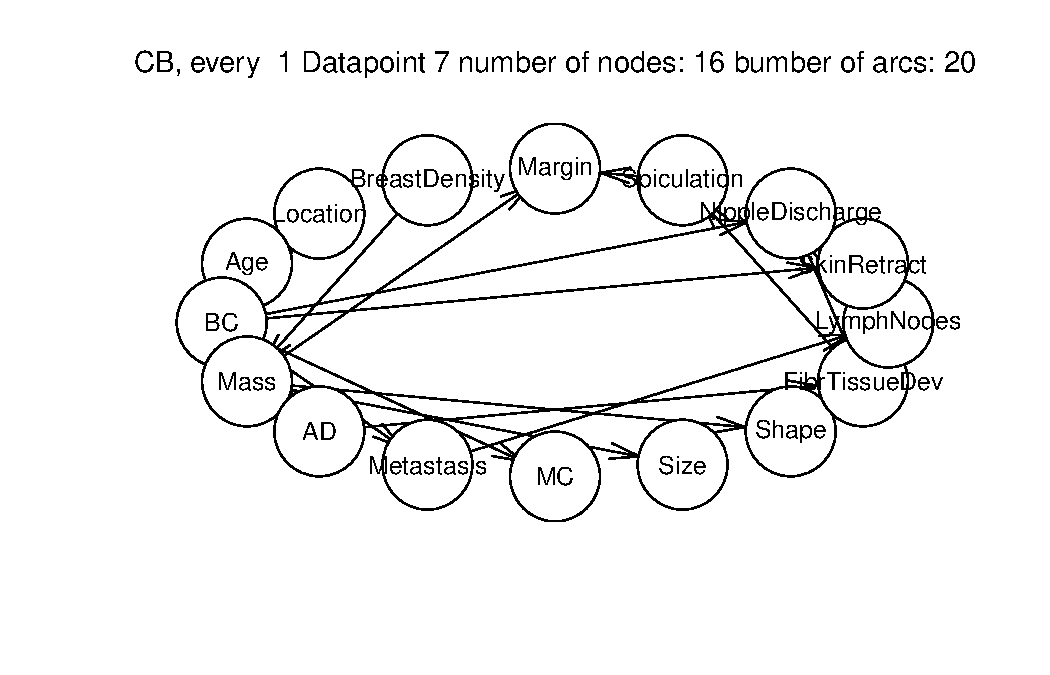
\includegraphics{BN_Ass2_files/figure-latex/unnamed-chunk-4-4.pdf}
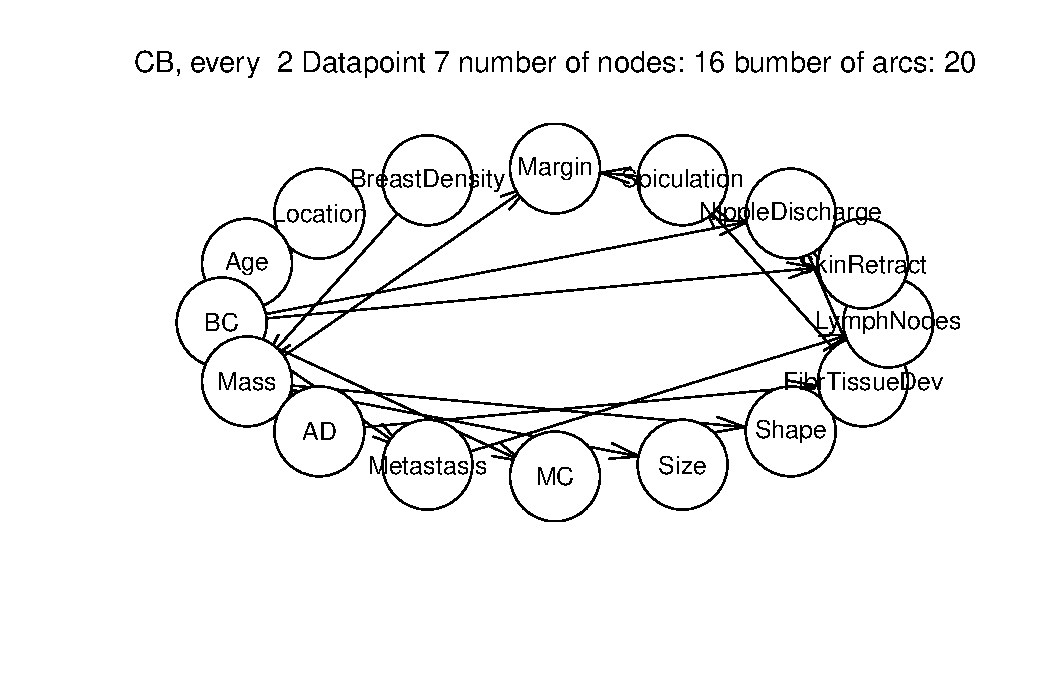
\includegraphics{BN_Ass2_files/figure-latex/unnamed-chunk-4-5.pdf}
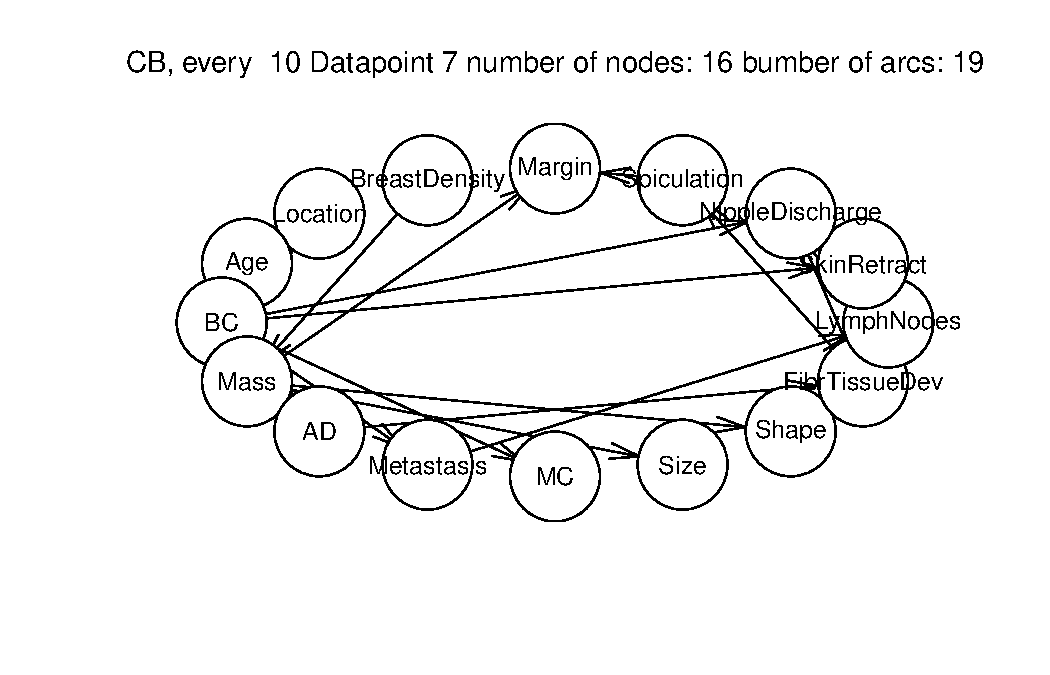
\includegraphics{BN_Ass2_files/figure-latex/unnamed-chunk-4-6.pdf}

\clearpage

\section{comparison to manually constructed bayes
network}\label{comparison-to-manually-constructed-bayes-network}

\section{3:define measures for quality of a learning algorithm in terms
of a known bayes network structure, motivate
definition}\label{define-measures-for-quality-of-a-learning-algorithm-in-terms-of-a-known-bayes-network-structure-motivate-definition}

Define measures that can be used to determine the quality of a learning
algorithm in terms of a known Bayesian network structure. Motivate the
definition of these measures

I have to be honest: I do not really understand that Question. Do the
authors suggest I find a measure that is original in describing the
quality of a bayesian Network? I'm sure that can't be true.

My measure for quality of the learning algorithm is Aruhga, which is the
Quotient between nodes and vertices.
\[Aruhga = \frac{Nodes}{Vertices}\]Arhuga is a binary measure with the
classes \{useful, not useful\}, depending on wether Aruhga falls inside
the interval {[}$\alpha , \beta${]}. $\alpha$ and $\beta$ are depending
heavily on the purpose and topic of the network and should normally be
defined by logical reasoning before constructing the network. However,
since the expert knowledge and necessary publications are not always
readily available, the author provides some default values with
$\alpha = 2.3$ and $\beta = 1.2/Nodes!$. Please note that Aruhga is a
measure of the connectivity of the network. values above alpha may
indicate that too many nodes are used, thus either weakening the
correlation between the single nodes OR bringing in Nodes that are not
relevant for each other. Networks with a value below beta indicate that
the network is highly connected which might reduce functionality and
also might point to a circular relationship between variables in the
real world that cannot be represented by a DAG.

\subsection{4:use measures to evaluate both classes of learning algs for
NHL
dataset}\label{use-measures-to-evaluate-both-classes-of-learning-algs-for-nhl-dataset}

Use these measures in order to evaluate the quality of both classes of
learning algorithms for the NHL dataset.

As we can see, the score based algorithm falls within a healthy 1.4 in
scores of Arugha. Thus we can conclude that the model might be useful

The constraint based algoritm however does not lie within the limits of
a ``useful'' Arugha, therefore we can conclude that it isn't very
useful. This seems to go well with the intuition one gets when looking
at the plot. Please note that some arcs are obstructed in the graph due
to the size of the nodes.

\begin{Shaded}
\begin{Highlighting}[]
\NormalTok{Tmp =}\StringTok{ }\KeywordTok{read.csv}\NormalTok{(}\StringTok{"nhl.csv"}\NormalTok{,}\DataTypeTok{nrows =} \DecValTok{5}\NormalTok{)}


\NormalTok{class =}\StringTok{ }\KeywordTok{rep}\NormalTok{(}\KeywordTok{list}\NormalTok{(}\StringTok{"factor"}\NormalTok{),}\KeywordTok{ncol}\NormalTok{(Tmp))}


\NormalTok{NHL =}\StringTok{ }\KeywordTok{read.csv}\NormalTok{(}\StringTok{"nhl.csv"}\NormalTok{,}\DataTypeTok{colClasses =} \NormalTok{class)}

\NormalTok{Tmp2<-}\StringTok{ }\KeywordTok{complete.cases}\NormalTok{(NHL) }\CommentTok{# only take complete cases}
\NormalTok{NHL <-}\StringTok{ }\NormalTok{NHL[Tmp2,]}


\NormalTok{NHLnet_sbl <-}\StringTok{ }\KeywordTok{tabu}\NormalTok{(NHL)}
\NormalTok{NHLnet_cbl <-}\StringTok{ }\KeywordTok{iamb}\NormalTok{(NHL)}


\NormalTok{numNodes =}\StringTok{ }\KeywordTok{length}\NormalTok{(NHLnet_sbl$nodes)}
\NormalTok{numArcs =}\StringTok{ }\KeywordTok{length}\NormalTok{(NHLnet_sbl$arcs[,}\DecValTok{1}\NormalTok{])}

\KeywordTok{plot}\NormalTok{(NHLnet_sbl, }\DataTypeTok{font.main =} \DecValTok{1}\NormalTok{, }\DataTypeTok{main =} \KeywordTok{paste}\NormalTok{(}\StringTok{"NHL SB, ibreaks = "}\NormalTok{, bins,  }\StringTok{"number of nodes:"} \NormalTok{, numNodes, }\StringTok{"bumber of arcs:"} \NormalTok{, numArcs))}
\end{Highlighting}
\end{Shaded}

\begin{figure}[htbp]
\centering
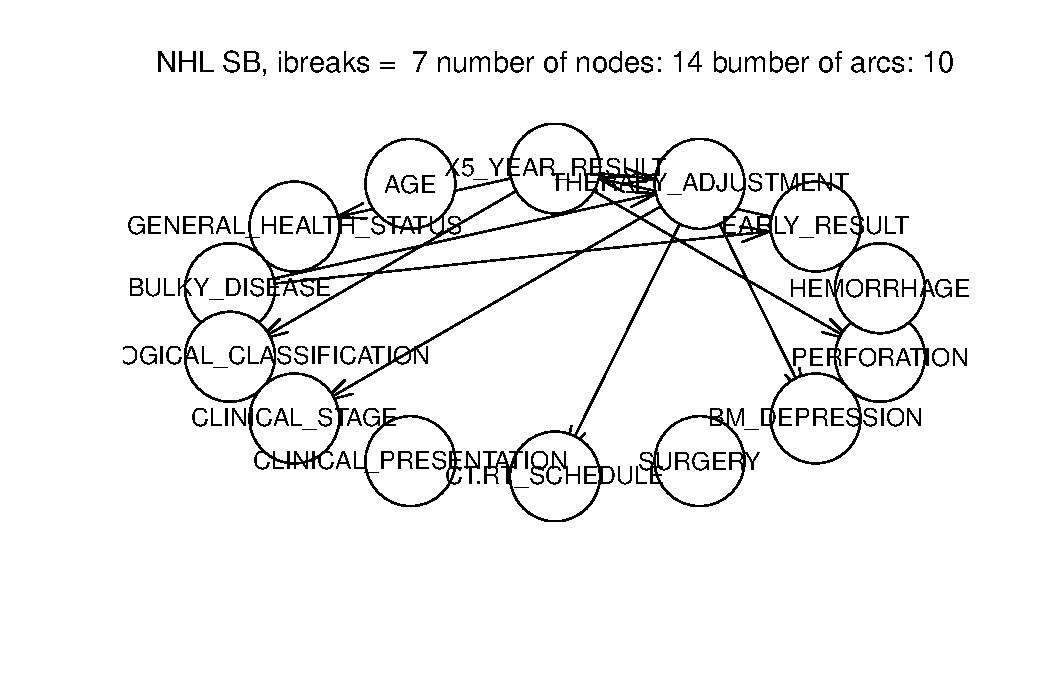
\includegraphics{BN_Ass2_files/figure-latex/unnamed-chunk-6-1.pdf}
\end{figure}

\begin{Shaded}
\begin{Highlighting}[]
\KeywordTok{print}\NormalTok{(}\KeywordTok{length}\NormalTok{(NHLnet_sbl$nodes)/}\KeywordTok{length}\NormalTok{(NHLnet_sbl$arcs[,}\DecValTok{1}\NormalTok{]))}
\end{Highlighting}
\end{Shaded}

\begin{verbatim}
## [1] 1.4
\end{verbatim}

\begin{Shaded}
\begin{Highlighting}[]
\NormalTok{numNodes =}\StringTok{ }\KeywordTok{length}\NormalTok{(NHLnet_cbl$nodes)}
\NormalTok{numArcs =}\StringTok{ }\KeywordTok{length}\NormalTok{(NHLnet_cbl$arcs[,}\DecValTok{1}\NormalTok{])}

\KeywordTok{plot}\NormalTok{(NHLnet_cbl, }\DataTypeTok{font.main =} \DecValTok{1}\NormalTok{, }\DataTypeTok{main =} \KeywordTok{paste}\NormalTok{(}\StringTok{"NHL CB, ibreaks = "}\NormalTok{, bins,  }\StringTok{"number of nodes:"} \NormalTok{, numNodes, }\StringTok{"bumber of arcs:"} \NormalTok{, numArcs))}
\end{Highlighting}
\end{Shaded}

\begin{figure}[htbp]
\centering
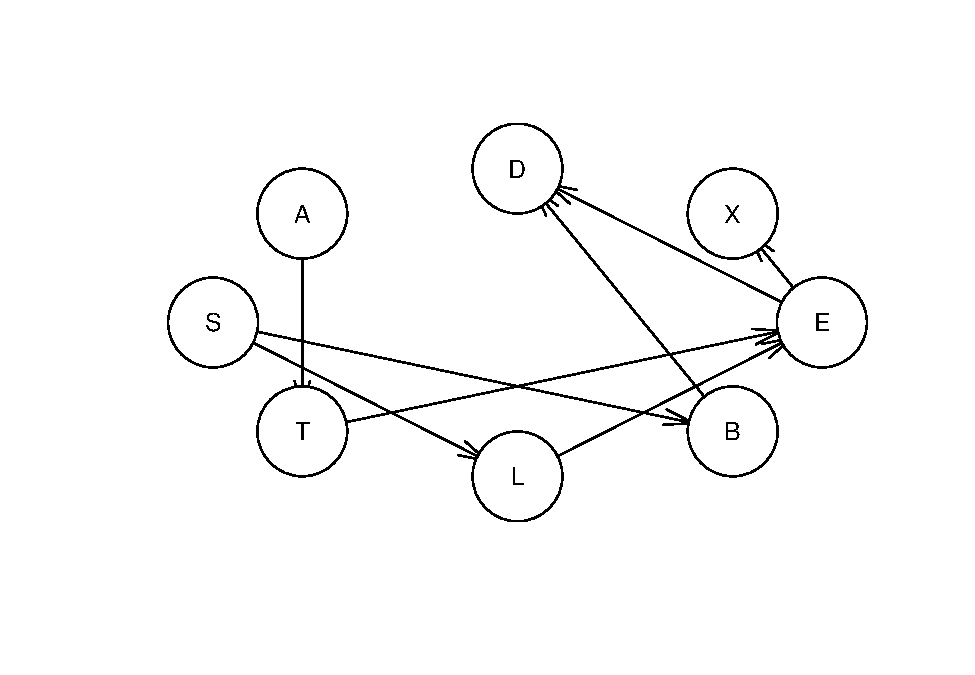
\includegraphics{BN_Ass2_files/figure-latex/unnamed-chunk-6-2.pdf}
\end{figure}

\begin{Shaded}
\begin{Highlighting}[]
\KeywordTok{print}\NormalTok{(}\KeywordTok{length}\NormalTok{(NHLnet_cbl$nodes)/}\KeywordTok{length}\NormalTok{(NHLnet_cbl$arcs[,}\DecValTok{1}\NormalTok{]))}
\end{Highlighting}
\end{Shaded}

\begin{verbatim}
## [1] 2.333333
\end{verbatim}

\subsection{5: compare margial prob distributions of learnt NHL bN with
those of the manually coinstructed
ones}\label{compare-margial-prob-distributions-of-learnt-nhl-bn-with-those-of-the-manually-coinstructed-ones}

Compare the marginal probability distributions of the learnt NHL
Bayesian network with those of the manually constructed network.

since constraint based aslgorithms do not necessarily produce directed
graphs, we will only examine score based algorithms.

\begin{Shaded}
\begin{Highlighting}[]
\NormalTok{fittedNHL =}\StringTok{ }\KeywordTok{bn.fit}\NormalTok{(NHLnet_sbl,NHL)}
\end{Highlighting}
\end{Shaded}

get the manually constructed network:

\begin{Shaded}
\begin{Highlighting}[]
\NormalTok{manual =}\StringTok{ }\KeywordTok{read.net}\NormalTok{(}\StringTok{"nhl.net"}\NormalTok{)}


\NormalTok{test <-}\StringTok{ }\KeywordTok{bn.net}\NormalTok{(manual)}
\KeywordTok{plot}\NormalTok{(test)}
\end{Highlighting}
\end{Shaded}

\begin{figure}[htbp]
\centering
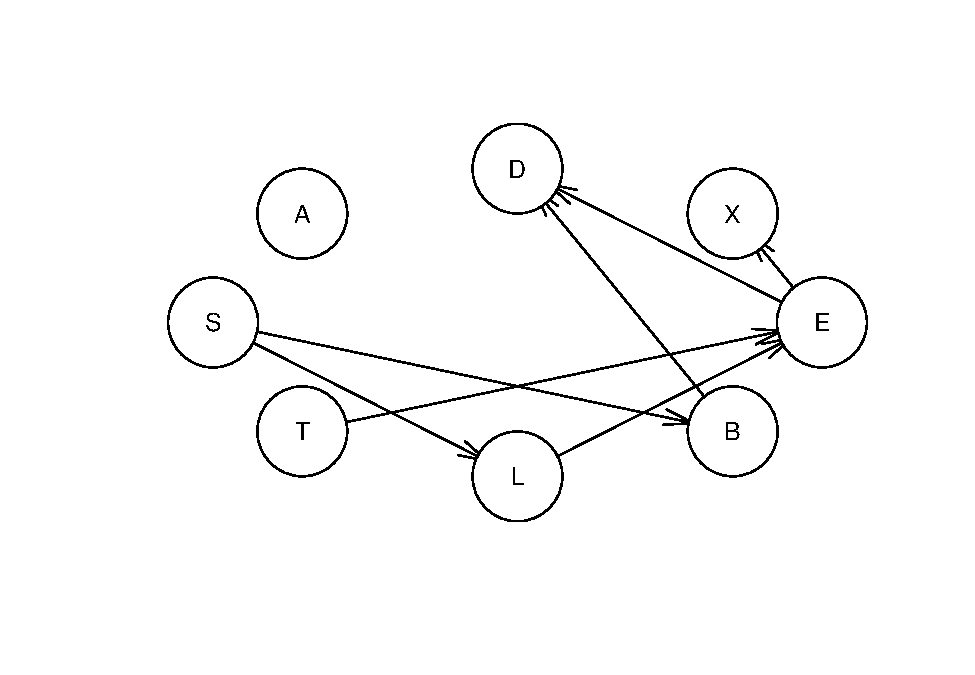
\includegraphics{BN_Ass2_files/figure-latex/unnamed-chunk-8-1.pdf}
\end{figure}

\begin{Shaded}
\begin{Highlighting}[]
\KeywordTok{print}\NormalTok{(}\KeywordTok{intersect}\NormalTok{(NHLnet_sbl$arcs,test$arcs))}
\end{Highlighting}
\end{Shaded}

\begin{verbatim}
## [1] "THERAPY_ADJUSTMENT"          "EARLY_RESULT"               
## [3] "BULKY_DISEASE"               "HISTOLOGICAL_CLASSIFICATION"
## [5] "GENERAL_HEALTH_STATUS"       "CLINICAL_STAGE"             
## [7] "PERFORATION"                 "BM_DEPRESSION"
\end{verbatim}

\begin{Shaded}
\begin{Highlighting}[]
\KeywordTok{print}\NormalTok{(}\KeywordTok{setdiff}\NormalTok{(}\KeywordTok{names}\NormalTok{(NHLnet_sbl$nodes),}\KeywordTok{names}\NormalTok{(test$nodes)))}
\end{Highlighting}
\end{Shaded}

\begin{verbatim}
## [1] "CT.RT_SCHEDULE" "X5_YEAR_RESULT"
\end{verbatim}

\begin{Shaded}
\begin{Highlighting}[]
\KeywordTok{print}\NormalTok{(}\KeywordTok{setdiff}\NormalTok{(}\KeywordTok{names}\NormalTok{(test$nodes),}\KeywordTok{names}\NormalTok{(NHLnet_sbl$nodes)))}
\end{Highlighting}
\end{Shaded}

\begin{verbatim}
## [1] "POST_SURGICAL_SURVIVAL" "HELICOBACTER_TREATMENT"
## [3] "CT_RT_SCHEDULE"         "POST_CT_RT_SURVIVAL"   
## [5] "ERADICATION"            "IMMEDIATE_SURVIVAL"    
## [7] "FIVE_YEAR_RESULT"       "HELICOBACTER_PYLORI"
\end{verbatim}

\begin{Shaded}
\begin{Highlighting}[]
\KeywordTok{print}\NormalTok{(}\KeywordTok{setdiff}\NormalTok{(NHLnet_sbl$arcs,test$arcs))}
\end{Highlighting}
\end{Shaded}

\begin{verbatim}
## [1] "X5_YEAR_RESULT" "CT.RT_SCHEDULE"
\end{verbatim}

\begin{Shaded}
\begin{Highlighting}[]
\KeywordTok{print}\NormalTok{(}\KeywordTok{setdiff}\NormalTok{(test$arcs,NHLnet_sbl$arcs))}
\end{Highlighting}
\end{Shaded}

\begin{verbatim}
##  [1] "POST_SURGICAL_SURVIVAL" "AGE"                   
##  [3] "HELICOBACTER_TREATMENT" "CLINICAL_PRESENTATION" 
##  [5] "SURGERY"                "CT_RT_SCHEDULE"        
##  [7] "POST_CT_RT_SURVIVAL"    "ERADICATION"           
##  [9] "HEMORRHAGE"             "IMMEDIATE_SURVIVAL"    
## [11] "HELICOBACTER_PYLORI"    "FIVE_YEAR_RESULT"
\end{verbatim}

\subsection{6: learn bayesian network from breast cancer daataset with
search and score or constraint based
algorithm}\label{learn-bayesian-network-from-breast-cancer-daataset-with-search-and-score-or-constraint-based-algorithm}

see section 2. This question seems redundant since the net has already
been trained in question 2 where it had to be compared in order of size
of data set. The net from question 2 will also be used in subsequent
sections.

\subsection{7: develop special purpose BN (NBN or TAN, see
.2)}\label{develop-special-purpose-bn-nbn-or-tan-see-.2}

\begin{Shaded}
\begin{Highlighting}[]
\NormalTok{netnb =}\StringTok{ }\KeywordTok{naive.bayes}\NormalTok{(a,}\StringTok{"BC"}\NormalTok{)}
\KeywordTok{plot}\NormalTok{(netnb, }\DataTypeTok{main =} \KeywordTok{c}\NormalTok{(}\StringTok{"NBN BC"}\NormalTok{))}
\end{Highlighting}
\end{Shaded}

\begin{figure}[htbp]
\centering
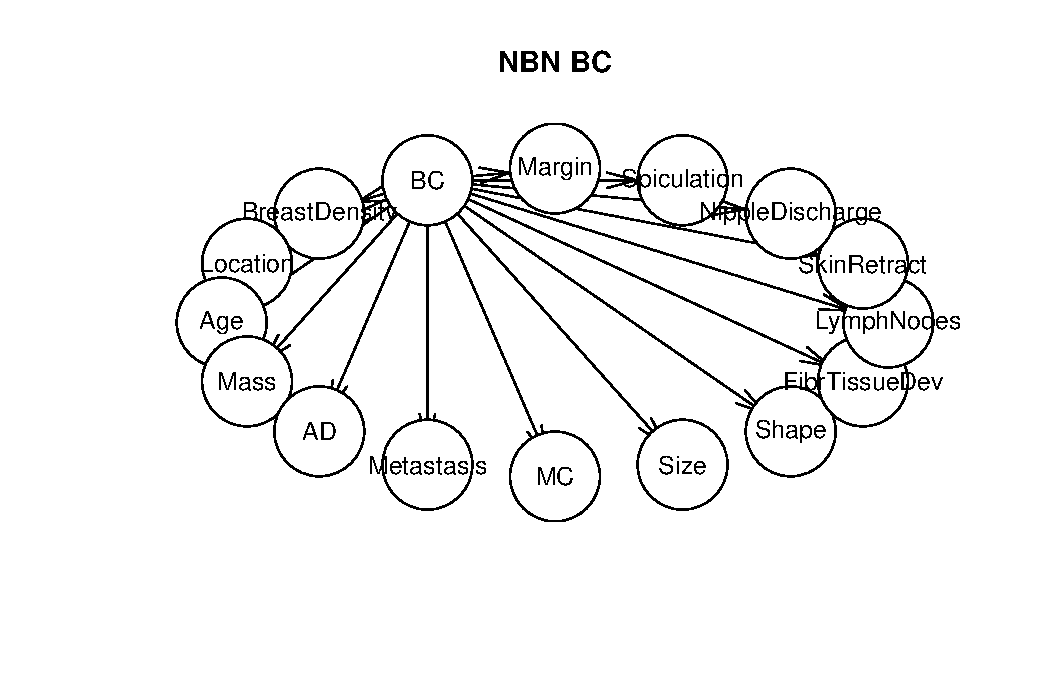
\includegraphics{BN_Ass2_files/figure-latex/unnamed-chunk-9-1.pdf}
\end{figure}

\begin{Shaded}
\begin{Highlighting}[]
\NormalTok{netnb2 <-}\StringTok{ }\KeywordTok{bn.fit}\NormalTok{(netnb,a)}
\end{Highlighting}
\end{Shaded}

\subsection{8:K compare BN and SPBN with manually constructed network in
terms of network structure, goodnes of fit scores (lkikelohood,\ldots{})
and accuracy measures such as misclassification error and ROC
(B.2)}\label{k-compare-bn-and-spbn-with-manually-constructed-network-in-terms-of-network-structure-goodnes-of-fit-scores-lkikelohood-and-accuracy-measures-such-as-misclassification-error-and-roc-b.2}

Compare the Bayesian network obtained by step (6) and the special
purpose Bayesian network from (7) with the manually constructed network
in Figure 2 in terms of network structure, goodness of fit scores (e.g.,
likelihood) and accuracy using measures such as misclassification error
and area under the ROC curve from cross-validation

\subsubsection{Read in manually constructed
network:}\label{read-in-manually-constructed-network}

\begin{Shaded}
\begin{Highlighting}[]
\NormalTok{manual =}\StringTok{ }\KeywordTok{read.net}\NormalTok{(}\StringTok{"bc.net"}\NormalTok{)}



\NormalTok{test <-}\StringTok{ }\KeywordTok{bn.net}\NormalTok{(manual)}
\KeywordTok{plot}\NormalTok{(test)}
\end{Highlighting}
\end{Shaded}

\begin{figure}[htbp]
\centering
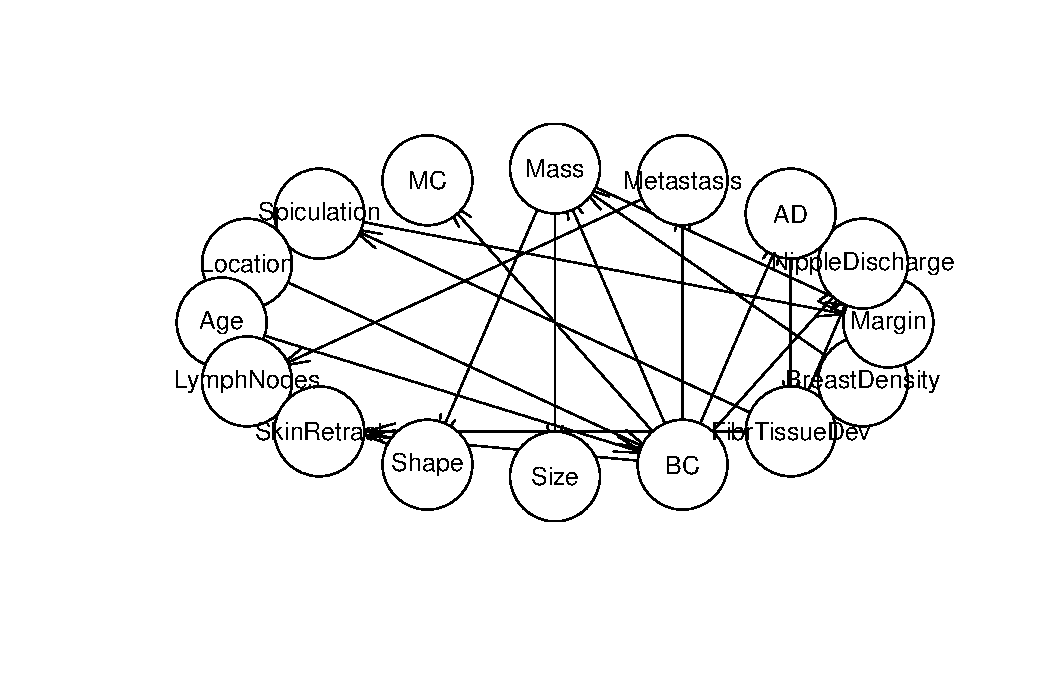
\includegraphics{BN_Ass2_files/figure-latex/unnamed-chunk-10-1.pdf}
\end{figure}

\begin{Shaded}
\begin{Highlighting}[]
\NormalTok{manual <-}\StringTok{ }\KeywordTok{bn.fit}\NormalTok{(test,BC)}
\end{Highlighting}
\end{Shaded}

\subsubsection{prediction error/cross
validation}\label{prediction-errorcross-validation}

\begin{Shaded}
\begin{Highlighting}[]
\NormalTok{nbncv <-}\StringTok{ }\KeywordTok{bn.cv}\NormalTok{(BC,netnb,}\DataTypeTok{loss=}\StringTok{"pred"}\NormalTok{,}\DataTypeTok{loss.args =} \KeywordTok{list}\NormalTok{(}\DataTypeTok{target=}\StringTok{"BC"}\NormalTok{),}\DataTypeTok{k=}\DecValTok{3}\NormalTok{)}
\end{Highlighting}
\end{Shaded}

\begin{verbatim}
## Warning in split.default(sample(n), seq_len(k)): Datenlänge ist kein
## Vielfaches der Split-Variablen
\end{verbatim}

\begin{Shaded}
\begin{Highlighting}[]
\NormalTok{nbncv}
\end{Highlighting}
\end{Shaded}

\begin{verbatim}
## 
##   k-fold cross-validation for Bayesian networks
## 
##   target network structure:
##    [Naive Bayes Classifier]
##   number of subsets:                     3 
##   loss function:                         Classification Error 
##   training node:                         BC 
##   expected loss:                         0.138
\end{verbatim}

\begin{Shaded}
\begin{Highlighting}[]
\NormalTok{bncv <-}\StringTok{ }\KeywordTok{bn.cv}\NormalTok{(BC,BC_sbl,}\DataTypeTok{loss=}\StringTok{"pred"}\NormalTok{,}\DataTypeTok{loss.args =} \KeywordTok{list}\NormalTok{(}\DataTypeTok{target=}\StringTok{"BC"}\NormalTok{),}\DataTypeTok{k=}\DecValTok{3}\NormalTok{)}
\end{Highlighting}
\end{Shaded}

\begin{verbatim}
## Warning in split.default(sample(n), seq_len(k)): Datenlänge ist kein
## Vielfaches der Split-Variablen
\end{verbatim}

\begin{Shaded}
\begin{Highlighting}[]
\NormalTok{bncv}
\end{Highlighting}
\end{Shaded}

\begin{verbatim}
## 
##   k-fold cross-validation for Bayesian networks
## 
##   target network structure:
##    [BreastDensity][Age][BC|Age][Location|BC][Mass|BreastDensity:BC][AD|BC]
##    [Metastasis|BC][MC|BC][Size|Mass][Shape|Mass][FibrTissueDev|AD]
##    [LymphNodes|Metastasis][SkinRetract|BC:FibrTissueDev]
##    [NippleDischarge|BC:FibrTissueDev][Spiculation|FibrTissueDev]
##    [Margin|Mass:Spiculation]
##   number of subsets:                     3 
##   loss function:                         Classification Error 
##   training node:                         BC 
##   expected loss:                         0.385
\end{verbatim}

\begin{Shaded}
\begin{Highlighting}[]
\NormalTok{Mncv <-}\StringTok{ }\KeywordTok{bn.cv}\NormalTok{(BC,test,}\DataTypeTok{loss=}\StringTok{"pred"}\NormalTok{,}\DataTypeTok{loss.args =} \KeywordTok{list}\NormalTok{(}\DataTypeTok{target=}\StringTok{"BC"}\NormalTok{),}\DataTypeTok{k=}\DecValTok{3}\NormalTok{)}
\end{Highlighting}
\end{Shaded}

\begin{verbatim}
## Warning in split.default(sample(n), seq_len(k)): Datenlänge ist kein
## Vielfaches der Split-Variablen
\end{verbatim}

\begin{Shaded}
\begin{Highlighting}[]
\NormalTok{Mncv}
\end{Highlighting}
\end{Shaded}

\begin{verbatim}
## 
##   k-fold cross-validation for Bayesian networks
## 
##   target network structure:
##    [Location][Age][BreastDensity][BC|Location:Age][MC|BC][AD|BC]
##    [Metastasis|BC][Mass|BC:BreastDensity][LymphNodes|Metastasis]
##    [Shape|Mass][Size|Mass][FibrTissueDev|AD][Spiculation|FibrTissueDev]
##    [SkinRetract|BC:FibrTissueDev][NippleDischarge|BC:FibrTissueDev]
##    [Margin|Spiculation:Mass]
##   number of subsets:                     3 
##   loss function:                         Classification Error 
##   training node:                         BC 
##   expected loss:                         0.385
\end{verbatim}

As clearly visible, the NB network has the lowest prediction loss,
whilöe the manually and algorithmically created networks have similar
values around \textasciitilde{}3.85 (probably light differences due to
rounding issues)

\subsubsection{ROC}\label{roc}

ROC fpr the BN

\begin{Shaded}
\begin{Highlighting}[]
\NormalTok{netcvfit1 =}\StringTok{ }\KeywordTok{as.grain}\NormalTok{(bncv[[}\DecValTok{1}\NormalTok{]]$fitted)}
\NormalTok{netcvfit2 =}\StringTok{ }\KeywordTok{as.grain}\NormalTok{(bncv[[}\DecValTok{2}\NormalTok{]]$fitted)}
\NormalTok{netcvfit3 =}\StringTok{ }\KeywordTok{as.grain}\NormalTok{(bncv[[}\DecValTok{3}\NormalTok{]]$fitted)}
\CommentTok{#head(netcvfit1)}

\NormalTok{nbntest1 =}\StringTok{ }\NormalTok{BC[bncv[[}\DecValTok{1}\NormalTok{]]$test, ]}
\NormalTok{nbntest2 =}\StringTok{ }\NormalTok{BC[bncv[[}\DecValTok{2}\NormalTok{]]$test, ]}
\NormalTok{nbntest3 =}\StringTok{ }\NormalTok{BC[bncv[[}\DecValTok{3}\NormalTok{]]$test, ]}
\CommentTok{#head(nbntest1)}


\NormalTok{pred_test1 =}\StringTok{ }\KeywordTok{predict}\NormalTok{(netcvfit1, }\DataTypeTok{response =} \KeywordTok{c}\NormalTok{(}\StringTok{"BC"}\NormalTok{), }\DataTypeTok{newdata =} \NormalTok{nbntest1,}
\DataTypeTok{predictors =} \KeywordTok{names}\NormalTok{(nbntest1)[-}\DecValTok{4}\NormalTok{], }\DataTypeTok{type =} \StringTok{"distribution"}\NormalTok{)}
\NormalTok{pred_test2 =}\StringTok{ }\KeywordTok{predict}\NormalTok{(netcvfit2, }\DataTypeTok{response =} \KeywordTok{c}\NormalTok{(}\StringTok{"BC"}\NormalTok{), }\DataTypeTok{newdata =} \NormalTok{nbntest2,}
\DataTypeTok{predictors =} \KeywordTok{names}\NormalTok{(nbntest2)[-}\DecValTok{4}\NormalTok{], }\DataTypeTok{type =} \StringTok{"distribution"}\NormalTok{)}
\NormalTok{pred_test3 =}\StringTok{ }\KeywordTok{predict}\NormalTok{(netcvfit3, }\DataTypeTok{response =} \KeywordTok{c}\NormalTok{(}\StringTok{"BC"}\NormalTok{), }\DataTypeTok{newdata =} \NormalTok{nbntest3,}
\DataTypeTok{predictors =} \KeywordTok{names}\NormalTok{(nbntest3)[-}\DecValTok{4}\NormalTok{], }\DataTypeTok{type =} \StringTok{"distribution"}\NormalTok{)}

\NormalTok{nbntest =}\StringTok{ }\KeywordTok{rbind}\NormalTok{(nbntest1,nbntest2,nbntest3)}

\CommentTok{#head(nbntest)}



\NormalTok{pred_test =}\StringTok{ }\KeywordTok{data.frame}\NormalTok{(}\KeywordTok{c}\NormalTok{(pred_test1$pred$BC[ ,}\DecValTok{2}\NormalTok{], pred_test2$pred$BC[ ,}\DecValTok{2}\NormalTok{],}
\NormalTok{pred_test3$pred$BC[ ,}\DecValTok{2}\NormalTok{]))}

\CommentTok{#head(pred_test)}
\CommentTok{#names(pred_test)}


\KeywordTok{colAUC}\NormalTok{(pred_test, nbntest[ ,}\DecValTok{4}\NormalTok{], }\DataTypeTok{plotROC =} \OtherTok{TRUE}\NormalTok{)}
\end{Highlighting}
\end{Shaded}

\begin{figure}[htbp]
\centering
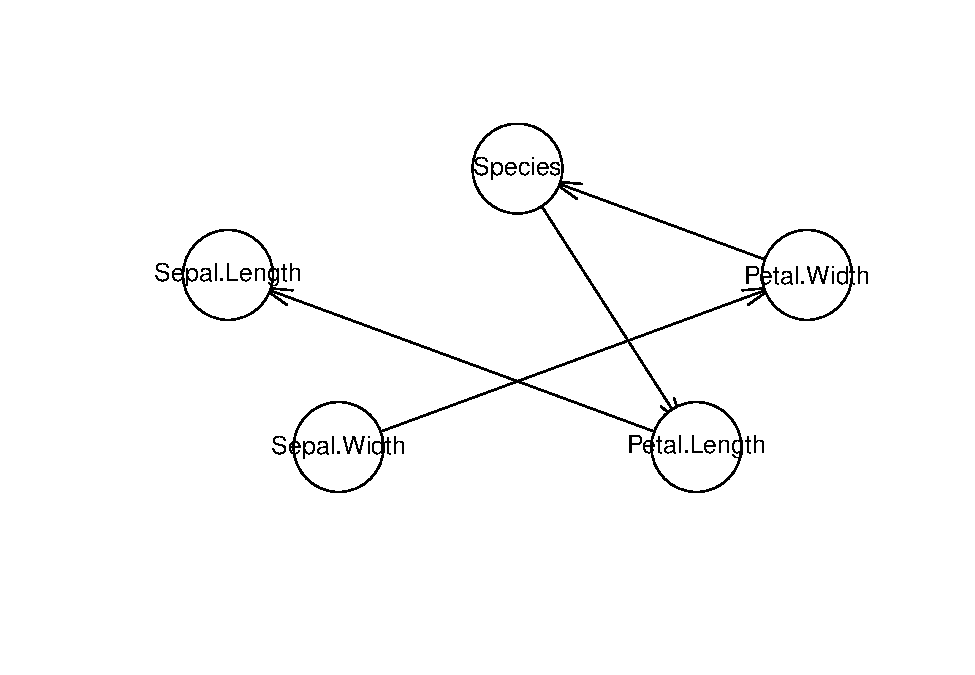
\includegraphics{BN_Ass2_files/figure-latex/unnamed-chunk-12-1.pdf}
\end{figure}

\begin{verbatim}
##                     c.pred_test1.pred.BC...2...pred_test2.pred.BC...2...pred_test3.pred.BC...
## Insitu vs. Invasive                                                                 0.9322321
## Insitu vs. No                                                                       0.9377949
## Invasive vs. No                                                                     0.9959340
\end{verbatim}

\begin{Shaded}
\begin{Highlighting}[]
\CommentTok{#title("test")}
\end{Highlighting}
\end{Shaded}

ROC for the NBN

\begin{Shaded}
\begin{Highlighting}[]
\NormalTok{netcvfit1 =}\StringTok{ }\KeywordTok{as.grain}\NormalTok{(nbncv[[}\DecValTok{1}\NormalTok{]]$fitted)}
\NormalTok{netcvfit2 =}\StringTok{ }\KeywordTok{as.grain}\NormalTok{(nbncv[[}\DecValTok{2}\NormalTok{]]$fitted)}
\NormalTok{netcvfit3 =}\StringTok{ }\KeywordTok{as.grain}\NormalTok{(nbncv[[}\DecValTok{3}\NormalTok{]]$fitted)}
\CommentTok{#head(netcvfit1)}

\NormalTok{nbntest1 =}\StringTok{ }\NormalTok{BC[nbncv[[}\DecValTok{1}\NormalTok{]]$test, ]}
\NormalTok{nbntest2 =}\StringTok{ }\NormalTok{BC[nbncv[[}\DecValTok{2}\NormalTok{]]$test, ]}
\NormalTok{nbntest3 =}\StringTok{ }\NormalTok{BC[nbncv[[}\DecValTok{3}\NormalTok{]]$test, ]}
\CommentTok{#head(nbntest1)}


\NormalTok{pred_test1 =}\StringTok{ }\KeywordTok{predict}\NormalTok{(netcvfit1, }\DataTypeTok{response =} \KeywordTok{c}\NormalTok{(}\StringTok{"BC"}\NormalTok{), }\DataTypeTok{newdata =} \NormalTok{nbntest1,}
\DataTypeTok{predictors =} \KeywordTok{names}\NormalTok{(nbntest1)[-}\DecValTok{4}\NormalTok{], }\DataTypeTok{type =} \StringTok{"distribution"}\NormalTok{)}
\NormalTok{pred_test2 =}\StringTok{ }\KeywordTok{predict}\NormalTok{(netcvfit2, }\DataTypeTok{response =} \KeywordTok{c}\NormalTok{(}\StringTok{"BC"}\NormalTok{), }\DataTypeTok{newdata =} \NormalTok{nbntest2,}
\DataTypeTok{predictors =} \KeywordTok{names}\NormalTok{(nbntest2)[-}\DecValTok{4}\NormalTok{], }\DataTypeTok{type =} \StringTok{"distribution"}\NormalTok{)}
\NormalTok{pred_test3 =}\StringTok{ }\KeywordTok{predict}\NormalTok{(netcvfit3, }\DataTypeTok{response =} \KeywordTok{c}\NormalTok{(}\StringTok{"BC"}\NormalTok{), }\DataTypeTok{newdata =} \NormalTok{nbntest3,}
\DataTypeTok{predictors =} \KeywordTok{names}\NormalTok{(nbntest3)[-}\DecValTok{4}\NormalTok{], }\DataTypeTok{type =} \StringTok{"distribution"}\NormalTok{)}

\NormalTok{nbntest =}\StringTok{ }\KeywordTok{rbind}\NormalTok{(nbntest1,nbntest2,nbntest3)}

\CommentTok{#head(nbntest)}



\NormalTok{pred_test =}\StringTok{ }\KeywordTok{data.frame}\NormalTok{(}\KeywordTok{c}\NormalTok{(pred_test1$pred$BC[ ,}\DecValTok{2}\NormalTok{], pred_test2$pred$BC[ ,}\DecValTok{2}\NormalTok{],}
\NormalTok{pred_test3$pred$BC[ ,}\DecValTok{2}\NormalTok{]))}

\CommentTok{#head(pred_test)}
\CommentTok{#names(pred_test)}


\KeywordTok{colAUC}\NormalTok{(pred_test, nbntest[ ,}\DecValTok{4}\NormalTok{], }\DataTypeTok{plotROC =} \OtherTok{TRUE}\NormalTok{)}
\end{Highlighting}
\end{Shaded}

\begin{figure}[htbp]
\centering
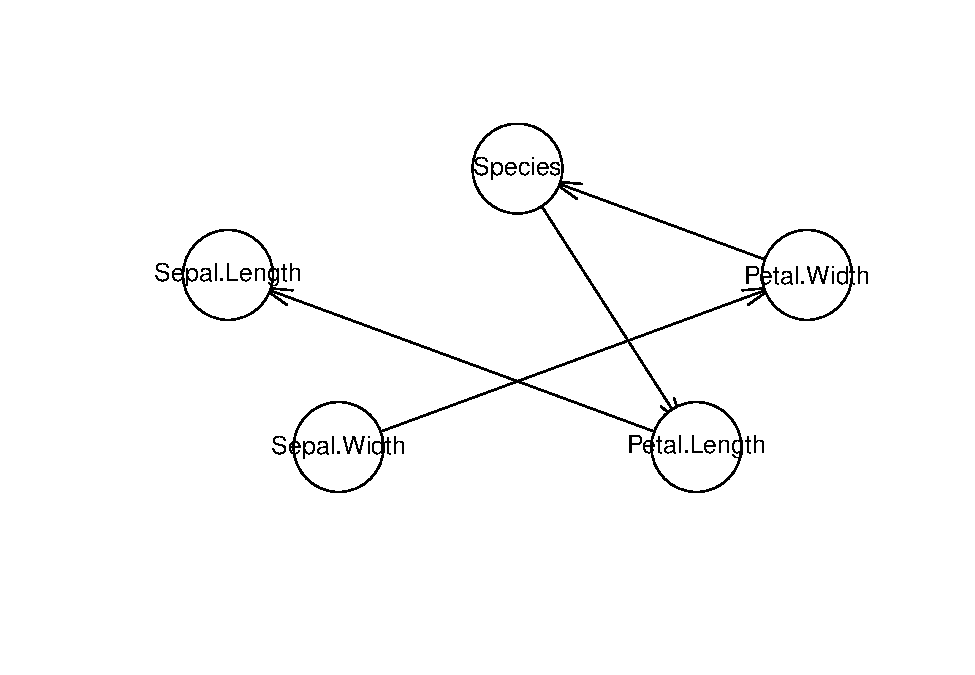
\includegraphics{BN_Ass2_files/figure-latex/unnamed-chunk-13-1.pdf}
\end{figure}

\begin{verbatim}
##                     c.pred_test1.pred.BC...2...pred_test2.pred.BC...2...pred_test3.pred.BC...
## Insitu vs. Invasive                                                                 0.9139066
## Insitu vs. No                                                                       0.9077385
## Invasive vs. No                                                                     0.9916419
\end{verbatim}

ROC fpor the manually created network

\begin{Shaded}
\begin{Highlighting}[]
\NormalTok{netcvfit1 =}\StringTok{ }\KeywordTok{as.grain}\NormalTok{(Mncv[[}\DecValTok{1}\NormalTok{]]$fitted)}
\NormalTok{netcvfit2 =}\StringTok{ }\KeywordTok{as.grain}\NormalTok{(Mncv[[}\DecValTok{2}\NormalTok{]]$fitted)}
\NormalTok{netcvfit3 =}\StringTok{ }\KeywordTok{as.grain}\NormalTok{(Mncv[[}\DecValTok{3}\NormalTok{]]$fitted)}
\CommentTok{#head(netcvfit1)}

\NormalTok{nbntest1 =}\StringTok{ }\NormalTok{BC[Mncv[[}\DecValTok{1}\NormalTok{]]$test, ]}
\NormalTok{nbntest2 =}\StringTok{ }\NormalTok{BC[Mncv[[}\DecValTok{2}\NormalTok{]]$test, ]}
\NormalTok{nbntest3 =}\StringTok{ }\NormalTok{BC[Mncv[[}\DecValTok{3}\NormalTok{]]$test, ]}
\CommentTok{#head(nbntest1)}


\NormalTok{pred_test1 =}\StringTok{ }\KeywordTok{predict}\NormalTok{(netcvfit1, }\DataTypeTok{response =} \KeywordTok{c}\NormalTok{(}\StringTok{"BC"}\NormalTok{), }\DataTypeTok{newdata =} \NormalTok{nbntest1,}
\DataTypeTok{predictors =} \KeywordTok{names}\NormalTok{(nbntest1)[-}\DecValTok{4}\NormalTok{], }\DataTypeTok{type =} \StringTok{"distribution"}\NormalTok{)}
\NormalTok{pred_test2 =}\StringTok{ }\KeywordTok{predict}\NormalTok{(netcvfit2, }\DataTypeTok{response =} \KeywordTok{c}\NormalTok{(}\StringTok{"BC"}\NormalTok{), }\DataTypeTok{newdata =} \NormalTok{nbntest2,}
\DataTypeTok{predictors =} \KeywordTok{names}\NormalTok{(nbntest2)[-}\DecValTok{4}\NormalTok{], }\DataTypeTok{type =} \StringTok{"distribution"}\NormalTok{)}
\NormalTok{pred_test3 =}\StringTok{ }\KeywordTok{predict}\NormalTok{(netcvfit3, }\DataTypeTok{response =} \KeywordTok{c}\NormalTok{(}\StringTok{"BC"}\NormalTok{), }\DataTypeTok{newdata =} \NormalTok{nbntest3,}
\DataTypeTok{predictors =} \KeywordTok{names}\NormalTok{(nbntest3)[-}\DecValTok{4}\NormalTok{], }\DataTypeTok{type =} \StringTok{"distribution"}\NormalTok{)}

\NormalTok{nbntest =}\StringTok{ }\KeywordTok{rbind}\NormalTok{(nbntest1,nbntest2,nbntest3)}

\CommentTok{#head(nbntest)}



\NormalTok{pred_test =}\StringTok{ }\KeywordTok{data.frame}\NormalTok{(}\KeywordTok{c}\NormalTok{(pred_test1$pred$BC[ ,}\DecValTok{2}\NormalTok{], pred_test2$pred$BC[ ,}\DecValTok{2}\NormalTok{],}
\NormalTok{pred_test3$pred$BC[ ,}\DecValTok{2}\NormalTok{]))}

\CommentTok{#head(pred_test)}
\CommentTok{#names(pred_test)}


\KeywordTok{colAUC}\NormalTok{(pred_test, nbntest[ ,}\DecValTok{4}\NormalTok{], }\DataTypeTok{plotROC =} \OtherTok{TRUE}\NormalTok{)}
\end{Highlighting}
\end{Shaded}

\begin{figure}[htbp]
\centering
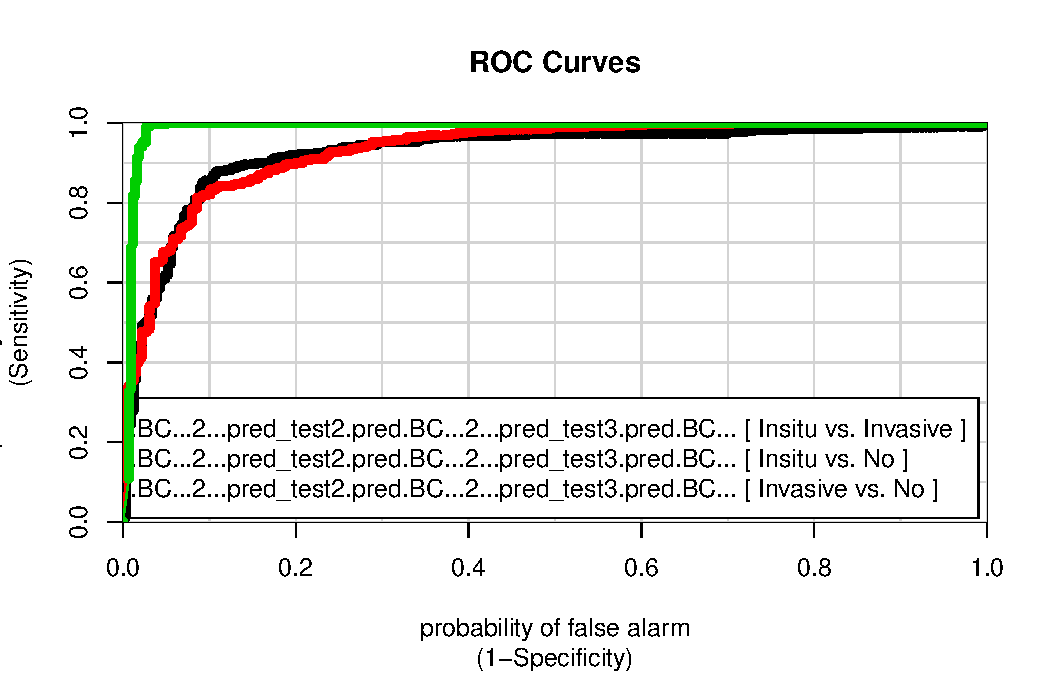
\includegraphics{BN_Ass2_files/figure-latex/unnamed-chunk-14-1.pdf}
\end{figure}

\begin{verbatim}
##                     c.pred_test1.pred.BC...2...pred_test2.pred.BC...2...pred_test3.pred.BC...
## Insitu vs. Invasive                                                                 0.9261455
## Insitu vs. No                                                                       0.9333495
## Invasive vs. No                                                                     0.9898786
\end{verbatim}

All the networks seem to perform pretty good, with scores around or
above .9. Best performance happens between invasive vs no, which seems
to match intuition since they are the very different.Best performance
overall seems to be held by the automatically created network with .93,
.937 and .995, while nbn and manally created network seem to have
different strengths, with nbn performing slightly better in invasive vs
no and the manually created slightly better in the others.

\footnote{Tobias Sing, Oliver Sander, Niko Beerenwinkel, Thomas Lengauer.
ROCR: visualizing classifier performance in R.
Bioinformatics 21(20):3940-3941 (2005). }

\newpage

Sing et al. (2005)

\newpage

\section{list of figures}\label{list-of-figures}

\listoffigures
\newpage

\section{references}\label{references}

\twocolumn

Sing, Tobias, Oliver Sander, Niko Beerenwinkel, and Thomas Lengauer.
2005. ``ROCR: visualizing Classifier Performance in R.''
\emph{Bioinformatics (Oxford, England)} 21 (20): 3940--1.
doi:\href{http://dx.doi.org/10.1093/bioinformatics/bti623}{10.1093/bioinformatics/bti623}.
\url{http://bioinformatics.oxfordjournals.org/content/21/20/3940.abstract}.

\end{document}
